\chapter{Research Background}

\todo[inline]{Talk about what is important for this thesis}
\todo[inline]{Check for overlaps with text in chapters 4,5,6,7,8.}

This chapter provides a background on the research streams related to this thesis. \Cref{sec:business-process} provides an overview on \gls{bpm} and its phases. \Cref{sec:software-development} gives an introduction on the main concepts of the software development process. \Cref{sec:project-oriented} illustrates a class of processes which belong to the intersection between software development and business process. 
The remaining sections further introduce research streams upon which to draw solutions for data-driven analyses of software development processes. \Cref{sec:process-mining} briefly describes the area of process mining. \Cref{sec:msr} describes contributions from the area of mining software repositories. \Cref{sec:visualization} provides an overview on the area of software visualization. \Cref{sec:text-mining} shortly describes the area of text mining, used for extracting knowledge from unstructured data. Finally, \Cref{sec:summary-of-relevant-techniques} summarizes these solutions. 
 

%This chapter is concerned with data-driven approaches used in literature to \emph{solutions}, which help tackling the problem of monitoring software development. Four disciplines provide the necessary theoretical and practical knowledge upon which this thesis is built. Thus, this chapter presents these four disciplines as follows. \Cref{sec:process-mining} briefly describes the area of process mining. \Cref{sec:msr} describes contributions from the area of mining software repositories. \Cref{sec:visualization} provides an overview on the area of software visualization. \Cref{sec:text-mining} shortly describes the area of text mining, used for extracting knowledge from unstructured data. Finally, \Cref{sec:summary-of-relevant-techniques} summarizes these solutions. 


\section{Business Process Management}
\label{sec:business-process}

\Glsfirst{bpm} is the discipline that oversees how work is performed in an organization to ensure consistent outcomes and exploit improvement opportunities~\citep{Dumas2018}. Rather than focusing on specific activities, events or decisions, \gls{bpm} focuses on how their interplay adds value to the organization and its customers. These chains of events are named \emph{processes}. More formally, a business process is set of activities that are performed in coordination in an organizational and technical
environment. These activities jointly realize a business goal~\citep{DBLP:books/sp/Weske19}.

%Its main change to previous way of conducting work is "process thinking" 
%Adam Smith -> Division of labour

Business process management aims at improving business processes following an iterative methodology which is refereed to as the \emph{BPM lifecycle}~\citep{Dumas2018}. It consists of six phases:
\begin{inparaenum}[\itshape i)]
	\item process identification,
	\item process discovery, 
	\item process analysis,
	\item process redesign,
	\item process implementation, and
	\item process monitoring.
\end{inparaenum}

In the \emph{process identification} phase a business problem is posed. The main goal of this phase is to define, enumerate and put into relation existing processes in the company. An artifact produced by this phase is a \emph{process architecture}. Such provides a guiding map for selecting which processes to further manage in the following \gls{bpm} phases. Typically, the processes that are most relevant to the posed business problem will be highlighted for further management.
In the \emph{process discovery} phase, processes are documented. Typically this is done via modeling the process in some modeling language (e.g., \gls{bpmn}\footnote{https://www.omg.org/bpmn}, Petri net~\citep{DBLP:journals/topnoc/LohmannVD09}, EPC~\citep{DBLP:books/wi/Dumas05/ScheerTA05}, \gls{yawl}~\citep{DBLP:journals/is/AalstH05}). The outcome of this phase is a set of so-called \emph{as-is} process models. 
In the \emph{process analysis} phase, the as-is processes are analyzed via qualitative and quantitative methods. The output of this phase is a collection of weaknesses in the as-is process along with their impact and estimated effort to address them.
In the \emph{process redesign} phase, the goal is to identify those changes to the existing process that address the previously identified issues and contribute to solving the posed business problem. Redesign changes are usually backed up by the analyses results Performance indicators are also used to measure performance of the processes. of the previous phase. An output of this phase is a redesigned process, which typically is also modeled into a \emph{to-be} process model.
In the \emph{process implementation} phase, the previously identified changes are implemented. This phase covers both changing the way work is performed in the organization and the set up and development of the IT systems required for the realization of the \emph{to-be} process. Special focus is here dedicated to the technical challenges of automating the new process with the goal of running it on a \gls{bpms}. Thus, the output of this phase consists of a set of executable process model. 
In the \emph{process monitoring} phase, various measures of the running process are collected. They provide the basis for analyzing the success of redesign, collecting new insights that emerged from the execution context and determining how well the new process is performing against defined quality/performance indicators. Deviations, issues and bottlenecks are here collected. They provide the starting point of a new iteration of the \gls{bpm} lifecycle.
\Cref{fig:bpm-lifecycle} summarizes the phases of the lifecycle and their interplay.

\begin{figure}
	\centering
	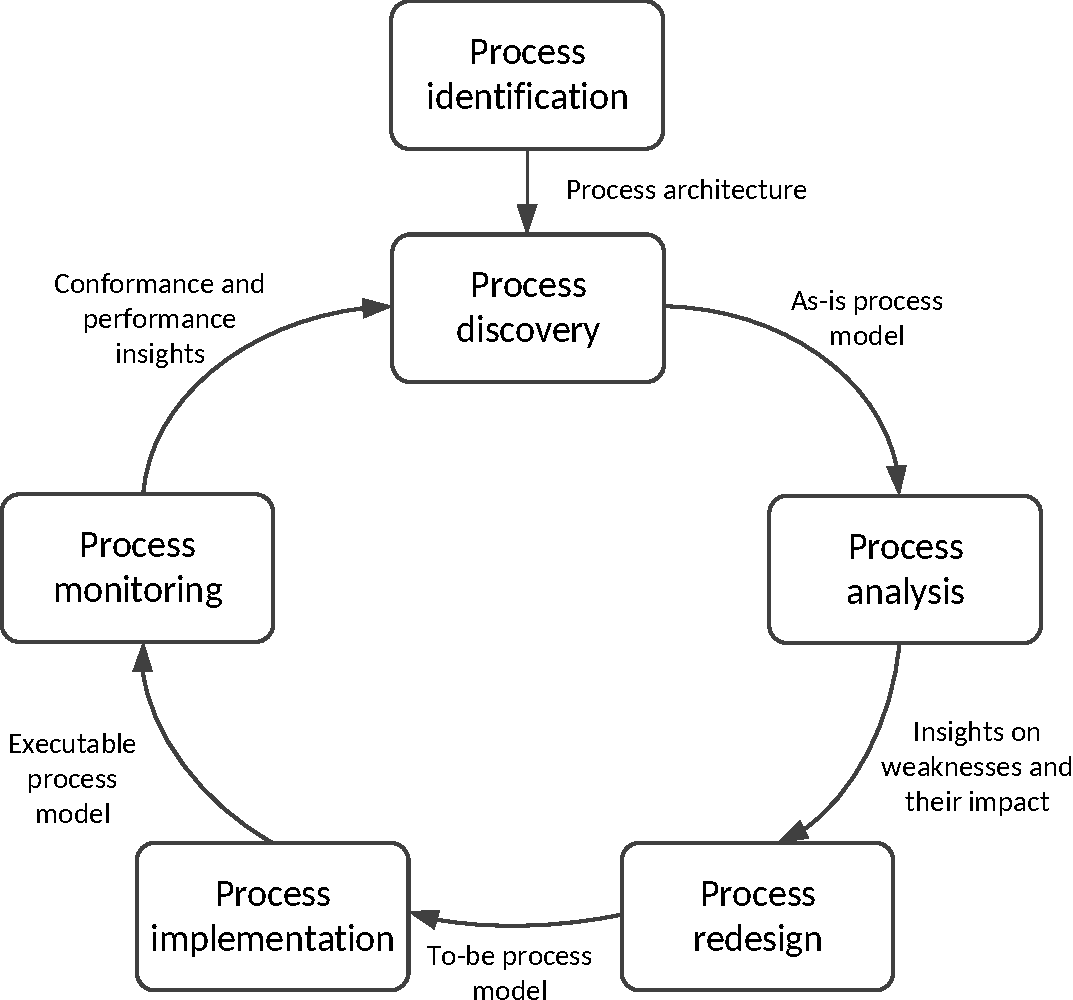
\includegraphics[width=0.8\linewidth]{figures/bpm-lifecycle}
	\caption[The BPM lifecycle]{The BPM lifecycle. Adapted from \cite[]{Dumas2018}}
	\label{fig:bpm-lifecycle}
\end{figure}

Coordination of work in business processes can be viewed from different perspectives. When analyzing business processes, a good characterization can be achieved with the following four perspectives~\citep{DBLP:books/sp/Aalst16}. 
First, the \emph{control-flow perspective} aims at capturing the all the possible paths in which activities may follow one-another in a process. Second, the \emph{organizational perspective} captures which actors (e.g., people, organizational units, roles) participate in the business process and how they interact with each other. Third, the \emph{case-perspective} captures the properties of specific process instances such as the evolution of certain data-objects, originators of the case, specific values of process variables, etc. Fourth, the time-perspective captures temporal information about the process, like when and how often certain activities occurred and what was their duration.


\section{Software Development Process}
\label{sec:software-development}

The software development process is a specific kind of process. Differently from standard business processes, it is run without referring to a process model. Rather in these cases, a methodology is followed. Popular methodologies in software development are Waterfall, Spiral, and Agile. Agile methods further refine into branches such as Scrum and Kanban. 

Commonalities between software development processes and business are the fact that they both describe and endeavor to organize work in such a way that can be measured and hence monitored and improved.  





\subsection{Software Development Methodologies}

Existing research shows that explicit knowledge defined by \glspl{sdm} improves productivity of software development enterprises and quality of the developed software. This is achieved by increasing enterprises’ ability to transfer knowledge between employees, systematically manage software development process, etc. \citep{avison2003information,DBLP:journals/iam/Fitzgerald98,hovelja2015exploring,DBLP:journals/tse/RiemenschneiderHD02}. However, it is not enough that an enterprise only describes its SDM in a document; the developers need to use it consistently in their everyday work. The use of SDM was often a topic of research in the last decades, since SDM adoption among software developers was relatively low and the developers often preferred different ad hoc approaches \citep{DBLP:journals/software/Aaen03,DBLP:journals/isj/Fitzgerald96,DBLP:journals/iam/HuismanI06}. 

The use of SDMs in enterprises can be analyzed with the help of different existing approaches (\citealp{DBLP:journals/imds/Aboelmaged10,venkatesh2000theoretical,DBLP:journals/behaviourIT/WangLH13}). One of the grounding theories in the field of SDM evaluation is diffusion of innovations theory \citep{rogers2010diffusion} according to which SDM is considered as innovation that developers adopt \citep{DBLP:journals/iam/Gallivan03,DBLP:journals/infsof/GreenHC05,DBLP:conf/caise/IivariH01}. To obtain information about the studied SDM and/or its elements the aforementioned studies focused on perceptions of different stakeholders, namely developers, managers, users, etc. to measure characteristics like level of use, assimilation, social and technical suitability, developer satisfaction and impact on performance \citep{atkinson1999project,cooper1990information,rogers2010diffusion,DBLP:journals/infsof/VavpoticB09,DBLP:journals/comsis/VavpoticH12}. Even better insight into SDM and/or its elements can be gained by comparing the perceptions of different stakeholders regarding the same SDM and/or its element \citep{hovelja2015exploring}. 

Another important theoretical development in the field was that SDM should be studied on the level of its constituent elements like activities, tools, roles, produced documents, etc. and not only as a whole. This improved the understanding of suitability of studied SDM elements for a certain development team and enabled comparison between the studied SDM elements. Thus, allowing enterprises to better pinpoint problematic elements of SDM, prepare focused improvements and examine the link between a specific SDM element and overall project success \citep{atkinson1999project,hovelja2015exploring}. Such development is in line with findings in the field of situational method engineering \citep{DBLP:journals/ejis/KarlssonA09,DBLP:conf/caise/RalyteDR03} that constructs a custom SDM from those SDM elements that fit with characteristics of certain development team and other situational factors (internal and external enterprise’s environment). 

Another potential source of information regarding development process emerged in recent years with widespread use of tools that support software development activities like issue tracking, requirements management, test management etc. Such tools store valuable data about actual execution of the development process and give us additional information about SDM and its elements thus importantly complementing stakeholder perceptions \citep{DBLP:journals/ese/ChoetkiertikulD17,DBLP:conf/msr/MantylaADGO16,DBLP:conf/msr/OrtuMDTTMA16,DBLP:conf/icse/OrtuDKM15}. 



\subsection{Software Repositories}

Software repositories store state data which reflect the work done on the software.

Version control systems are one type of software repository that is used to track the different versions of a file. 


Tracking is required not only explicitly as part of some activities but also to comply with norms and regulations that may require some evidence of the actions being performed in the organization. Documents are usually free of format or contain tables, at best. The unstructuredness of data makes it difficult to monitor processes and check rules on them. A starting point for analysis of project-oriented processes can be data logs %generated for  %usually consist of subversion projects
that are stored in Software Configuration Management (SCM) systems that help tracking the evolution of data and restore information if needed~\citep{voinea_open_2006}.
However, hundreds of versions of thousands of files are common in a single project~\citep{voinea_multiscale_2006}, which makes it impractical to browse this data manually.

%We focus on project mining motivated by a real case scenario in the scope of the SHAPE research project\footnote{\url{http://ai.wu.ac.at/shape-project/}}.
%The data log is provided by a Version Control Systems (VCS) whose information is not subdivided into traces related to process instances but consists of a hierarchy of work streams associated with individual files being added, modified or deleted in a subversion repository.

Let us see an example inspired by a real scenario of a process to write a project proposal that uses a Version Control System (VCS) to store the data. The project history, and hence, the data produced, starts when people begin to work on the proposal, which involves a description of the project goals and milestones, a division of tasks into work packages, an estimation of cost and resources required, etcetera. This information is spread in the repository over several folders containing different documents, which are later merged into a single file. If the proposal is accepted, the first step is to organize a kickoff meeting and assign specific resources to the work packages. A hierarchical set of folders is then created in the repository in order to store the information generated for each work package. As the project evolves over time, resources contribute by adding, removing or modifying information to the VCS repository. %\todo{Should answer point 3 on the review-list: Missing concrete examples of the need to “prove compliance to rules and regulations”. Which important rules and regulations will the analysis help comply with?} 
Project evolution is guided by specific norms that impose the execution of predefined steps. For instance, the European norm EN5016 requires a preliminary \gls{ram} analysis to support targets. 
%Data stored in the VCS can be used to prove compliance to rules and regulations of the domain. For instance, in the railway industry, 

Table~\ref{tab:bpm2015example} depicts an excerpt of the log data generated, where the first column (on the left hand side) indicates the commit identifier, the second column indicates the person who committed changes, the third column indicates the commit date, %the fourth column shows (optional) descriptive information to clarify the scope of the changes performed
and the fourth column indicates the files affected and the type of action performed among added (A), modified (M) and deleted (D).
For the sake of simplicity, the table shows the log data of a specific time period and the actions related to a specific task, namely, $\defineExample$. That task was assigned to resource X % after a project meeting. %, when a part of project members asked for a toy example to better understand the problem domain.
and was supervised by resource Y and, later on, also by resource Z.
%An extract from the log concerning this period, that shows some crucial steps in the \emph{example} task, is reported on table \ref{tab:example}. Comments were left out from this representation, since at the current state we don't delve into them.

\begin{table}[bt]
	\caption{Excerpt from VCS log data for the referenced time period }
	\label{tab:bpm2015example}
	%\scriptsize
	{
		%	\renewcommand{\arraystretch}{1.3}
		\centering
		%\fontfamily{phv}\fontseries{mc}\selectfont
		\begin{tabular}{m{.8cm} m{1.5cm} m{3cm} p{5.8cm}}
			%\hline\noalign{\smallskip}
			%\hline
			\toprule
			\textbf{CID}	 & \textbf{Resource} & \textbf{Date} & \textbf{List of changes} \\
			%\noalign{\smallskip}
			%\hline
			%\noalign{\smallskip}
			%\hline
			\midrule
			%\noalign{\smallskip}
			\multirow{2}{*}{1} & \multirow{2}{*}{Y} & \multirow{2}{*}{2014-11-12~11:57:46} & A /example \\
			& & & A \slash example\slash SHAPE\slash\-ToyStation\-Example.docx \\ \midrule %\hdashline
			
			%\multirow{2}{*}{205} & \multirow{2}{*}{X} & \multirow{2}{*}{2014-11-14 16:26:23} & A /example/ToyStation.bpmn \\
			%& & & A /example/ToyStation.png \\ \hline %\hdashline
			
			\ldots & \ldots & \ldots & \ldots \\ \midrule
			
			%\noalign{\smallskip}
			\multirow{2}{*}{3} & \multirow{2}{*}{X} & \multirow{2}{*}{2014-11-14 16:34:07} & M /example/ToyStation.bpmn\\
			& & & M /example/ToyStation.png \\ \midrule%\hdashline
			
			%\multirow{7}{*}{207} & \multirow{7}{*}{X} & \multirow{7}{*}{2014-11-27 14:18:59} & M /example/SHAPE-ToyStation-Example.docx \\
			%& & & D /example/ToyStation.bpmn \\
			%& & & M /example/ToyStation.png \\
			%& & & A /example/ToyStation\_0Loop.bpmn \\
			%& & & A /example/ToyStation\_1Loop.bpmn \\
			%& & & A /example/ToyStation\_nLoop.bpmn \\
			%& & & A/example/ToyStation\_old.bpmn\\ \hline
			
			%\ldots & \ldots & \ldots & \ldots \\ \hline
			
			%\noalign{\smallskip}
			4 & W & 2014-12-15 13:49:11 & D /example/Download \\ \midrule %\hdashline
			
			%\noalign{\smallskip}
			5 & W & 2015-01-08 16:06:41 & A /example/Download2\\ \midrule %\hdashline
			
			%\noalign{\smallskip}
			\multirow{2}{*}{6} & \multirow{2}{*}{X} & \multirow{2}{*}{2015-01-13 11:47:09} & M /example/ToyStation\_0Loop.bpmn\\
			& & & M /example/ToyStation\_nLoop.bpmn \\ \midrule %\hdashline
			
			%\noalign{\smallskip}
			\multirow{2}{*}{7} & \multirow{2}{*}{Z} & \multirow{2}{*}{2015-01-16 16:50:29} & A /example/ToyStation\_0Loop.pdf\\
			& & & A /example/ToyStation-feedbackZ.pdf\\ \bottomrule %\hdashline
		\end{tabular}\\ 
	}
\end{table}


Existing frameworks, such as Subversion or Git, allow to access their logs in different ways. However, the covered information is limited to (roughly) that depicted in Table~\ref{tab:bpm2015example}. Especially for big projects that are frequently updated over a large period of time, these logs are complex to analyze.
Therefore, the problem to address is how to analyze and visualize the information produced in project-oriented business processes such that it can be represented in an understandable and manageable way by project experts and
enable, a.o., the automation of mechanisms for compliance checking.
The following properties of project-oriented process logs must be taken into account to achieve this goal: (i) VCS repositories consist of a hierarchy of folders and files which are logically organized such that work is grouped in a specific way; (ii) process activities are not registered in VCS log entries. Therefore, such information must be inferred by reasoning on the repository structure and/or the content of the log entries; (iii) the granularity of the events is unknown a priori and it needs to be defined before analyzing the data.


\todo[inline]{Harmonize:}

In this work, we focus on a specific class of project-oriented business processes, namely software development processes. These processes share some common characteristics. First, they involve various resources with different roles. In the simplest case, we can distinguish \emph{project managers} and \emph{project participants}. Project managers are responsible for managing the development process and supervising the work of the project participants, who in turn are responsible for specific work tasks. Second, such processes are usually subject to constraints in terms of cost, time and quality, which is mostly associated with the performance of each of the work tasks. Third, the project participants work on a plethora of artifacts, which are logically organized in a hierarchical structure, with complex interdependencies among them.
Given these characteristics, it is the goal of the project manager to organize the software development process in such a way that the work on different files and tasks reflects the complex interdependencies, the constraints and the available participants. Therefore, it is important for the manager to understand the \emph{work history} of the process in order to monitor the progress systematically.

%project specifies the tasks to be performed considering a hierarchy of files, within a limited period of time, and with a limited set of project participants, for achieving a specific goal, typically the release of a new version of a software. Best practices are often used to properly organize the work according, for instance, to good modularization principles. However, monitoring whether this or other guidelines are followed in the actual development process is not easy, due to the lack of an overarching process that defines the work.

%Project managers are interested in an understanding of the running project from a macro level. Useful information is concerns:
%\begin{inparaenum}[\itshape i)]
%	\item project structure;
%	\item profiles of users;
%	\item and the work history.
%\end{inparaenum} Existing tools in software development can help project managers to monitor and control these perspectives individually. For instance, CVS

%Nevertheless, these tools lack on information considering the work process reflected in the artifacts, i.e. artifact evolution, and a dependency among them beyond the structural provided by the hierarchy. Moreover, it is common to have hundreds of versions of thousands of files in a single project, which makes it impractical to browse this data manually.

% Please add the following required packages to your document preamble:
% \usepackage{booktabs}
% \usepackage{graphicx}
% \usepackage[normalem]{ulem}
% \useunder{\uline}{\ul}{}
%\vspace*{-.3cm}

%\newcommand{\colsep}{\hspace*{52pt}}
\begin{table*}[]
	\caption{An excerpt of a VCS log data}
	\label{tab:vcs-log-data}
	\setlength{\tabcolsep}{6pt}
\centering
%\resizebox{\textwidth}{!}{%
%\begin{tabular}{@{ }cm{.7cm}m{2cm}m{4.8cm}m{7cm}@{ }}
\begin{tabular}{@{ }cm{1.8cm}m{1.6cm}m{4cm}m{7cm}@{ }}
\toprule
Id & \begin{tabular}[c]{@{}l@{}}Project \\ Participant\end{tabular} & Date                          & Comment                          & Diff                                                                                                                                                                                                                                                                                   \\ \midrule \rowcolor{lightgray}
1          & John    & 2017-01-31 12:16:30 & Create readme file                   & \begin{tabular}[c]{@{}l@{}}diff --git a/README.md b/README.md\\ @@ -0,0 +1 @@\\+\# StoryMiningSoftwareRepositories\end{tabular}                                                                                                                                                          \\
2          & Mary    & 2017-02-01 10:13:51 & Add a license                   & \rowsep \begin{tabular}[c]{@{}l@{}}diff --git a/README b/README\\ @@ -1,0 +2,3 @@\\ +The MIT License (MIT)\\ +\\ +Copyright (c) 2015 Mary+\end{tabular}                                                                                                                                     \\
\rowcolor{lightgray} 3          & Paul    & 2017-02-02 16:10:22 & Updated the requirements.               & \rowsep \begin{tabular}[c]{@{}l@{}}diff --git a/README.md b/README.md\\ @@ -1,4 +1,5 @@ \\ + \# string 1, string 2, string 3\\ \\ diff --git a/requirements.txt b/requirements.txt\\ @@ -0,0 +1 @@\\ +The software must solve the problems\end{tabular} \\
4          & Paul    & 2017-02-02 15:00:02 & Implement new requirements & \rowsep \begin{tabular}[c]{@{}l@{}}diff --git a/model.java b/model.java\\ @@ -1,9 +1,10 @@ \\ {+public static methodA()\{int newVal=0;}\\ @@ -21,10 +23,11 @@\\ + "1/0",,"0/0",\\ \\ diff --git a/test.java b/test.java\\ @@ -0,0 +1,2 @@\\ +//test method A\\ +testMethodA()\end{tabular}  \\ \bottomrule
\end{tabular}%
%}
\end{table*} 


\section{Project-Oriented Business Process}
\label{sec:project-oriented}

Project-oriented business processes are a category of business processes which have the following characteristics. 

They are usually one shot. When run twice, the second instance differs from the first. 

These kind of processes have specific requirements for monitoring. 

These processes are suited to describe plans. These plans can regard for example, the delivery of a software systems at a specified time and under specific restrictions of budget. 


%Business process management plays an important role for improving the performance and compliance of various types of processes. In practice, many processes are executed with clear guidelines and regulatory rules, but without an explicit centralized control imposed by a process engine. In particular, it is often important to exactly know when which work was done. This is, for instance, the case for complex engineering processes in which different parties are involved. We refer to this class of processes as project-oriented business processes.
%
%Such project-oriented business processes are difficult to control due to the lack of a centralized process engine. However, there are various unstructured pieces of information available to analyze and monitor their progress. One type of data that are often available these processes is event data from version control systems (VCS). While process mining techniques provide a useful perspective on how such event data can be analyzed, they do not produce output that is readily organized according to the project orientation of these processes.
%
%In this thesis, we define formal concepts for capturing project-oriented processes. These concepts provide the foundation for us to develop an automatic discovery technique which we refer to as \emph{project mining}. The output of our project mining algorithm is organized according to the specific structure typically encountered in project-oriented business processes. With this work, we extend the field of process mining towards the coverage of this specific type of business process.

The class of processes that we discuss in this paper are long-term engineering projects. These processes have specific requirements for monitoring. First, they are executed only once according to the specific needs of a particular project, and only partially according to recurring process descriptions. Second, they involve various actors that typically document their work in a semi-structured way using text and tables. Third, work in the project is usually subject to constraints regarding the start and end and the temporal order. Fourth, there is typically no process engine controlling the execution. Fifth, even though these limitations in terms of traceability exist, there are usually strong requirements in terms of tracking when which work was conducted.

%Unlike other types of business processes, the processes we consider here
%representing such projects are specifically tailored to customer needs the specific needs of the project, and there is

In line with these observations, a \textit{project-oriented business process} can be defined as an ad-hoc plan that specifies the tasks to be performed within a limited period of time and with a limited set of resources for achieving a specific goal. Unlike repetitive business processes for which notations such as \gls{bpmn}~\citep{bpmn2_stable} or \gls{epc}~\citep{vanderaalst_formalization_1999} are commonly used, project-oriented business processes may be properly represented with \gls{pert} or GANTT models. The concept is illustrated in Fig.~\ref{fig:bpm2015problem}.


\begin{figure}[htbp!]
	\centering
	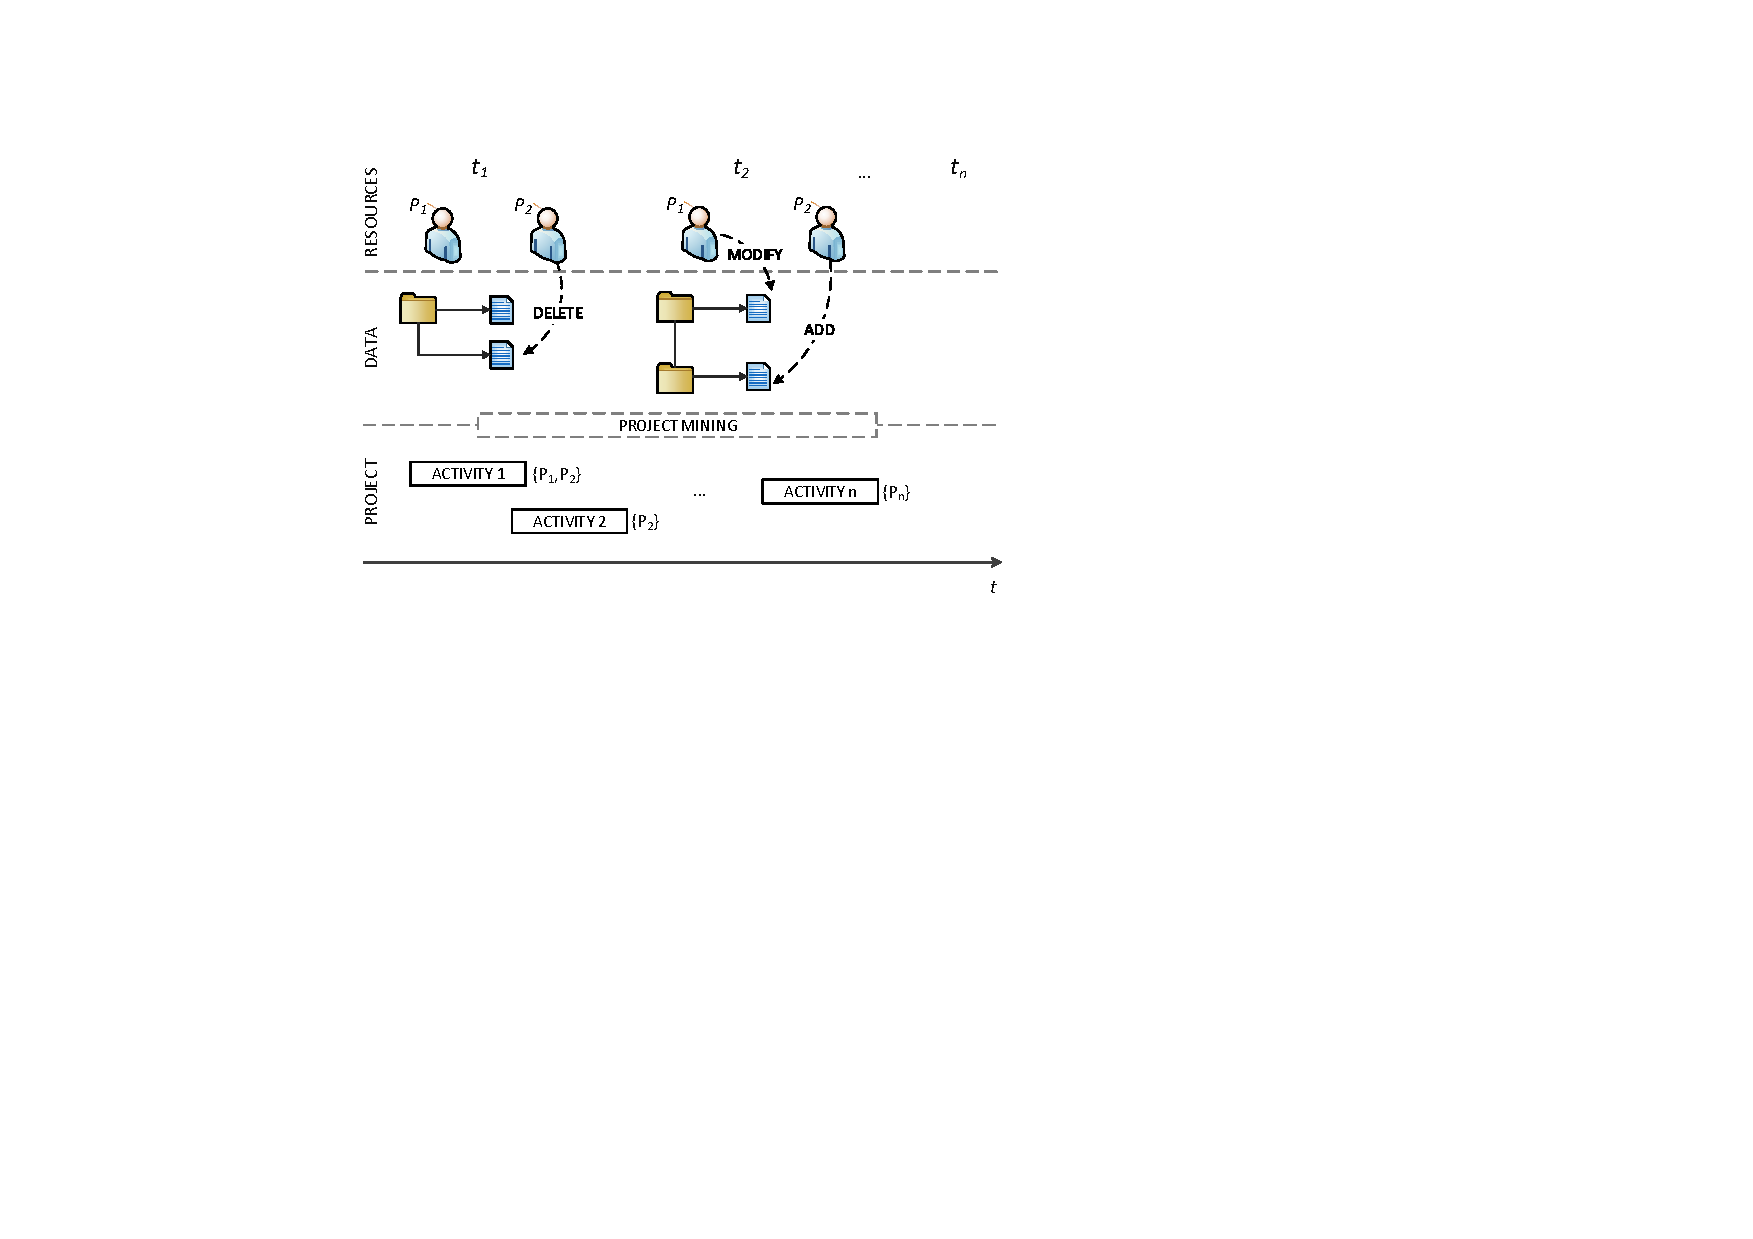
\includegraphics[width=.8\textwidth]{bpm2015/imgs/ProjectMining.pdf}
	\caption{Gap between User-Generated Artifacts and Project-Activities}
	\label{fig:bpm2015problem}
\end{figure}






